\chapter{Accepttest}

\begin{longtabu} to \linewidth{@{}l l l X[l]@{}}


 Version &    Dato &    Ansvarlig &    Beskrivelse\\[-1ex]
    \midrule
    0.1 &    28-09-2015 &   MHNK og MBA &    Oprettelse og udfyldelse af Accepttest \\[-1ex]
    0.2 &    30-09-2015 &   ABH &    Tilrette accepttest  \\[-1ex]
    0.3 &    08-10-2015 &   Alle &    Tilrette efter review med Grp. 1 \\[-1ex]
    0.4	&	15-10-2015	&	MBA 	 &	Indskrevet i LaTex \\
	0.5	&	20-10-2015	&	MHNK &	Tilretning \\
    0.6	&	26-11-2015	&	MHNK &	Retning af hele accepttesten. Konsekvent med stavemåder \\
    0.7 &	10-12-2015  & DHC, ABH, AJF & Rettelser i forhold til slutprodukt \\
    0.8	&	13-12-2015	&	MHNK &	Færdiggørelse efter accepttest. Indskrivning af godkendelser. Oprettelse og skrivning af problemrapport \\
   
    
\label{version_Systemark}
\end{longtabu}

\section{Accepttest af Use Cases}

\section{Indledning}
Accepttestene skal vise om produktet lever op til de standarder vi har sat op for, at den aktivt kan indgå i en forskningssituation. 
Accepttesten er en opfølgning af kravspecifikation, som har til formål at sikre at alle kravene er overholdt. Der vil blive testet både på hovedscenarier samt på undtagelser. Det er målsætningen, at disse test sikrer produktets kvalitet, idet produktet vil blive afprøvet før det tages i brug. Derfor er det accepttestens ansvarsfunktion, at godkende de opsatte delmål for produktet hvad angår både funktionalitet samt ikke-funktionelle krav. \\
Data der benyttes til målingerne fås fra In Vitro, der i form af tryk genererer et fysiologisk tryk. Brugergrænsefladen er det som forskeren initierer med, altså hvorfra systemet aktiveres. Brugergrænsefladen forkortes til GUI. Den benyttede Database er en lokal database. 
Når der i feltet Godkendt er et flueben, betyder det at testen er godkendt. Hvis der er et flueben i parenteser, betyder det at den er delvis godkendt. 


%Use case 1 acceptest
\subsection{Use Case 1}
Indsæt beskrivelse og figurer med NI-DAQ, Analog discovery og transduceren.
Det forventes for Use Case 1 , at forskeren har fået påmonteret det væskefyldte kateter samt tændt for apparaturet. 

\begin{longtabu} to \linewidth{@{}l r X[j]@{}} %UC1%
	\toprule
	Test af Use Case 1  				&&	Foretag nulpunktsjustering\\
	Scenarie 							&&	Hovedscenarie\\
	Prækondition 						&&	Blodtryksmålesystemet er monteret korrekt.
Forskeren har tændt for Blodtryksmåleren og pop-up vindue for nulpunktsjustering er åbent\\ \midrule
\end{longtabu}


\begin{longtabu} to \linewidth{@{} c X[l] X[l] X[j] l@{}}
    ~ &	\textbf{Handling} &    \textbf{Forventet observation/resultat} &		\textbf{Faktisk observation/resultat} &    \textbf{Godkendt}\\[-1ex]
    \midrule
    ~ &\textit{Hovedscenarie} & ~ & ~ &
    \\ \midrule
    1. & Forsker trykker på Foretag-knap &   Systemet foretager nulpunktsjustering, hvorefter vinduet lukker &      Som forventet foretager systemet nulpunktsjustering, hvorefter vinduet lukker, når forsker har trykket på Foretag-knap &	{\Huge \checkmark}	
 \\ \bottomrule
 
\caption{Accepttest af Use Case 1}\\
\label{AT_UC1}
\end{longtabu}

%%%%%%%%%%%%%%%%%%%%%%%%%%%%%%%%%%%%%%%%%%%%%%%%%%%%%%%%%%%%%%%%%%%%%
\subsection{Use Case 2}
\begin{longtabu} to \linewidth{@{}l r X[l]@{}} %UC2%
	\toprule
	Test af Use Case 2  				&&	Bestem kalibreringskoefficient\\
	Scenarie 							&&	Hovedscenarie\\
	Prækondition 						&&	Hardware er monteret ved 50 mmHg på væskesøjlen og er tilkoblet en computer med WaveForm.  
\\ \midrule
\end{longtabu}

\begin{longtabu} to \linewidth{@{} c X[l] X[l] X[j] l@{}}

\setlength{\textfloatsep}{10pt plus 1.0pt minus 2.0pt}
    ~ &	\textbf{Handling} &    \textbf{Forventet observation/resultat} &		\textbf{Faktisk observation/resultat} &    \textbf{Godkendt}\\[-1ex]
    \midrule
    ~ &\textit{Hovedscenarie} & ~ & ~ &
    \\ \midrule
   	1. 	& 	Output spænding fra hardware aflæses i WaveForm	&  Output aflæses til 1 V +/- 30\% &  I WaveForm aflæses output til 1 V +/- 30\%     &	{\Huge \checkmark}	
    \\
    2. & Beregning foretages ud fra formlen $ \frac{50}{output} = koefficient$   &  Koefficenten beregnes til 50 +/- 30\%   &  Som forventet beregnes koefficenten til 50 +/- 30  &		{\Huge \checkmark}
	\\
	3. & Forsker indtaster beregnet kalibreringskoefficient i konfigurations XML-fil   &  Koefficenten står i XML-fil  &  Koefficenten står i XML-fil  &		{\Huge \checkmark}
	\\
	4. & Kalibreringskoefficient kan tilgås af systemet   &  Sammenlign værdierne i listen råData(findes i IndhentDAQData) med den viste graf på GUI &  Sammenlign værdierne i listen råData(findes i IndhentDAQData) med den viste graf på GUI  &		{\Huge \checkmark}
 \\ \bottomrule
 
\caption{Accepttest af Use Case 2}\\
\label{AT_UC2}
\end{longtabu}

%%%%%%%%%%%%%%%%%%%%%%%%%%%%%%%%%%%%%%%%%%%%%%%%%%%%%%%%%%%%%%%%%%%%

\subsection{Use Case 3}
\begin{longtabu} to \linewidth{@{}l r X[l]@{}} %UC2%
	\toprule
	Test af Use Case 3  				&&	Start måling\\
	Scenarie 							&&	Hovedscenarie\\
	Prækondition 						&&	Blodtryksmålesystemet er monteret korrekt.
Forskeren har tændt for Blodtryksmåleren. UC1 er kørt succesfuldt

\\ \midrule
\end{longtabu}


\begin{longtabu} to \linewidth{@{} c X[l] X[l] X[j] l@{}}
    ~ &	\textbf{Handling} &    \textbf{Forventet observation/resultat} &		\textbf{Faktisk observation/resultat} &    \textbf{Godkendt}\\[-1ex]
    \midrule
    ~ &\textit{Hovedscenarie} & ~ & ~ &
    \\ \midrule
    1. & Forsker indtaster Forsøgsnavn &   Systemet tilgængeliggør Start Måling-knap  &   Når forsker indtaster Forsøgsnavn, så gør systemet Start Måling-knap tilgængelig   & {\Huge \checkmark}
    \\
    2. & Filteret signal er valgt per default af systemet &    Radiobutton til filtret signal er checket af  & Det ses at Radiobutton til filtret signal er chefcket af  &	{\Huge \checkmark}
    \\
    3. & Forsker trykker på Start Måling-knap på GUI  &    Signal vises i graf på GUI   & Når forsker trykker på Start Måling-knap, vises signalet i graf på GUI  &		{\Huge \checkmark}
    \\
    4. & Systolisk og diastolisk blodtryk samt puls bliver vist i bokse på GUI &    GUI udskriver systoliske, diastoliske og puls værdier på GUI  &  GUI udskriver systoliske og diastoliske værdier på GUI. GUI udskriver ikke puls\footnote{Se problemrapport}  &	{\Huge (\checkmark)}	
    \\
    \midrule
    ~ &\textit{Udvidelse 1: Forsker vælger filtreret/ ufiltreret signal} & ~ & ~ &
    \\ \midrule
    1. & Forsker vælger ufiltreret signal &   Grafen viser det ufiltreret signal  &   Forsker vælger ufiltreret signal og grafen viser det ufiltreret signal    &		{\Huge \checkmark}
    \\
    2. & Forsker vælger filtreret signal &   Grafen viser det filtreret signal  &   Forsker vælger filtreret signal og grafen viser det filtreret signal    &		{\Huge \checkmark}
 \\ 
 \bottomrule
 
\caption{Accepttest af Use Case 3}\\
\label{AT_UC3}
\end{longtabu}


%%%%%%%%%%%%%%%%%%%%%%%%%%%%%%%%%%%%%%%%%%%%%%%%%%%%%%%%%%%%%%%%%%%%

\subsection{Use Case 4}
\begin{longtabu} to \linewidth{@{}l r X[l]@{}} %UC2%
	\toprule
	Test af Use Case 4  				&&	Gem data\\
	Scenarie 							&&	Hovedscenarie\\
	Prækondition 						&&	Blodtryksmålesystemet er monteret korrekt.
Forskeren har tændt for Blodtryksmåleren. Use Case 1 er kørt succesfuldt, Use Case 3 kører


\\ \midrule
\end{longtabu}


\begin{longtabu} to \linewidth{@{} c X[l] X[l] X[j] l@{}}
    ~ &	\textbf{Handling} &    \textbf{Forventet observation/resultat} &		\textbf{Faktisk observation/resultat} &    \textbf{Godkendt}\\[-1ex]
    \midrule
    ~ &\textit{Hovedscenarie} & ~ & ~ &
    \\ \midrule
    1. & Forsker trykker på Start Gem-knap  &   Start Gem-knap bliver highlightet med blå kant  & Når forsker trykker på Start Gem-knap bliver den highlightet med blå kant     &		{\Huge \checkmark}
    \\
    2. & Forsker trykker på Stop Gem-knap for at stoppe med at gemme &    Filnavnet(forsøgsnavn\_Id) bliver vist i tekstboks GUI  & Når forsker trykker på Stop Gem-knap for at gemme bliver filnavnet(forsøgsnavn\_Id) vist i tekstboks i GUI   &	{\Huge \checkmark}
    \\
    3. & Forsker trykker på Gem-knap for at stoppe med at gemme  &    Det fremgår af GUI at data er gemt i Database   &  Når forsker trykker på Gem-knap for at stoppe med at gemme, fremgår det af GUI at data er blevet gemt i Database &		{\Huge \checkmark}
    \\
    \midrule
    ~ &\textit{Undtagelse 1: Forsker trykker på Stop Måling-knap} & ~ & ~ &
    \\ \midrule
    1. & Forsker trykker på Stop Måling-knap til et givent tidspunkt  &   Grafen på GUI fastholdes og datostempel på seneste indlagte data aflæses i databasens tabel. Tiderne sammenlignes  &  Når forsker trykker på Stop Måling-knap til et givent tidspunkt, fastholdes grafen på GUI og datostempel på seneste indlagte data aflæses i databasens tabel, hvor efter tiderne sammenlignes     &		{\Huge \checkmark}
 \\ \bottomrule
 
\caption{Accepttest af Use Case 4}\\
\label{AT_UC4}
\end{longtabu}

%%%%%%%%%%%%%%%%%%%%%%%%%%%%%%%%%%%%%%%%%%%%%%%%%%%%%%%%%%%%%%%%%%%%

\subsection{Use Case 5}
\begin{longtabu} to \linewidth{@{}l r X[l]@{}} %UC2%
	\toprule
	Test af Use Case 4  				&&	Stop måling\\
	Scenarie 							&&	Hovedscenarie\\
	Prækondition 						&&	Blodtryksmålesystemet er monteret korrekt.
Forskeren har tændt for Blodtryksmåleren. Use Case 1 er kørt succesfuldt, Use Case 3 kører

\\ \midrule
\end{longtabu}


\begin{longtabu} to \linewidth{@{} c X[l] X[l] X[j] l@{}}
    ~ &	\textbf{Handling} &    \textbf{Forventet observation/resultat} &		\textbf{Faktisk observation/resultat} &    \textbf{Godkendt}\\[-1ex]
    \midrule
    ~ &\textit{Hovedscenarie} & ~ & ~ &
    \\ \midrule
    1. & Forsker trykker på Stop Måling-knap  &   Målingen stoppes og blodtryksgrafen fastholdes  &   Forsker trykker på Stop Måling-knap og målingen stoppes og blodtryksgrafen fastholdes    &		{\Huge \checkmark}
    \\
    
 \\ \bottomrule
 
\caption{Accepttest af Use Case 5}\\
\label{AT_UC5}
\end{longtabu}

%%%%%%%%%%%%%%%%%%%%%%%%%%%%%%%%%%%%%%%%%%%%%%%%%%%%%%%%%%%%%%%%%%%%



\newpage
\section{Accepttest af ikke-funktionelle krav}

\begin{longtabu} to \linewidth{@{} c X[l] X[l] X[j] X[j] l@{}}
	Krav nr. & Krav & Test & Forventet resultat & Resultat & Godkendt
	\\[-1ex] \midrule
	
	1. & Blodtryks-måleren skal indeholde en Start Måling-knap til at igangsætte målingerne. & Kør Use Case 1 og 3 & Start Måling-knap er på GUI & Use Case 1 og 3 køres og der er en Start Måling-knap på GUI & {\Huge \checkmark}
	\\ 
	\midrule
	
	2. & Blodtryks-måleren skal indeholde en Stop Måling-knap, hvorfra måling kan stoppes. & Kør Use Case 1 og 3 & Stop Måling-knap er på GUI & Use Case 1 og 3 køres og der er en Stop Måling-knap på GUI & {\Huge \checkmark}
	\\ 
	\midrule
	
	3. & Blodtryks-måleren skal indeholde en Start Gem-knap til påbegyndelses af at gemme måling i Database & Kør Use Case 1 og 3 & Start Gem-knap er på GUI & Use Case 1 og 3 køres og der er en Start Gem-knap på GUI & {\Huge \checkmark}
	\\ 
	\midrule
	
	4. & Blodtryks-måleren skal indeholde en Stop Gem-knap til påbegyndelses af at gemme måling i Database & Kør Use Case 1 og 3 & Stop Gem-knap er på GUI & Use Case 1 og 3 køres og der er en Stop Gem-knap på GUI & {\Huge \checkmark}
	\\ 
	\midrule
	
	5. & Blodtryks-måleren skal indeholde en tekstboks til forsøgsnavn, hvori forsker indtaster det pågældende forsøgsnavn & Kør Use Case 1 og 3 & Tekstboks til forsøgsnavn er på GUI & Use Case 1 og 3 køres og der er en tekstboks til forsøgsnavn, hvori forsker indtaster det pågældende forsøgsnavn  & {\Huge \checkmark}
	\\ 
	\midrule
	
	
	6. & Blodtryks-måleren skal indeholde radiobutton til filtreret signal, denne skal være default valget & Kør Use Case 1 og 3 & Radiobutton til filtreret signal er på GUI & Use Case 1 og 3 køres og der er en radiobutton til filtreret signal, der er valgt per default  &  {\Huge \checkmark}
	\\ 
	\midrule
	
	
	
	7. & Blodtryks-måleren skal indeholde radiobutton til ufiltreret signal & Kør Use Case 1 og 3 & Radiobutton til ufiltreret signal er på GUI & Use Case 1 og 3 køres og der er en radiobutton til ufiltreret signal &  {\Huge \checkmark}
	\\ 
	\midrule
	
	
	
	8. & Blodtryks-måleren skal indeholde tekstbokse til puls, systolisk og diastolisk blodtryk, som vises med op til tre cifre & Kør Use Case 1 og 3 & Systolisk-boks, diastolisk-boks og puls-boks er på GUI & Use Case 1 og 3 køres og der er tekstbokse, der indeholder puls, systolisk og diastolisk blodtryk, som vises med op til tre cifre  & {\Huge \checkmark}
	\\ 
	\midrule
	
	9. & Blodtryks-måleren skal indeholde en tekstboks, som viser filnavn(forsøgsnavn og id) på målingen, efter måling er gemt & Kør Use Case 1 og 3 & Tekstboks til Filnavn er på GUI & Use Case 1 og 3 køres og der er en tekstboks, der viser filnavn(forsøgsnavn og id) på målingen, efter måling er gemt  & {\Huge \checkmark}
	\\ 
	\midrule
	
	10. & GUI’en skal se ud som på figur \ref{fig:Skitse af GUI} i KS & GUI’en ser ud som figur \ref{fig:Skitse af GUI} i KS & GUI’en ser ud som figur \ref{fig:Skitse af GUI} i KS & GUI’en ser ud som figur \ref{fig:Skitse af GUI} i KS & {\Huge \checkmark}
	\\ 
	\midrule
	
	
	11. & Forskeren skal kunne starte en default-måling maksimalt 30 sekunder efter systemet er startet & Systemet er åben samtidigt startes et stopur. Efter tryk på Start Måling-knap og målingen er startet stoppes uret & Måling er startet og stopuret viser mindre end 30 sekunder & Systemet er åbent og samtidigt med at et stopur startes trykkes der på Start Måling-knap og når målingen er startet stoppes uret. Forskeren kunne altså indenfor 30 sekunder, efter systemet er startet, starte en default-måling  & {\Huge \checkmark}
	\\ 
	\midrule
	
	
	12. & Det skal maksimalt tage 5 timer at gendanne systemet (MTTR - Mean Time To Restore) & Kan ikke testes på prototypen & Kan ikke testes på prototypen & Kan ikke testes på prototypen & {\Huge \checkmark}
	\\ 
	\midrule
	
	
	
	13. & Systemet skal have en oppetid uden nedbrud på minimum 1 måned (720 timer) (MTBF - Mean Time Between Failure) & Kan ikke testes på prototypen & Kan ikke testes på prototypen & Kan ikke testes på prototypen & {\Huge \checkmark}
	\\ 
	\midrule
	
	
	
	14. & Systemet skal have en oppetid/køretid på: $\dfrac{MTBF}{MTBF+MTTR}*100=99,31\%$ & Kan ikke testes på prototypen & Kan ikke testes på prototypen & Kan ikke testes på prototypen & {\Huge \checkmark}
	\\ 
	\midrule
	
	
	15. & Blodtryks-måleren skal, indenfor 3 sekunder, kunne vise systolisk og diastolisk blodtryk via graf. Dette accepteres med en tolerance på +/- 15 \% & Kør Use Case 1 og 3. Der trykkes på Start Måling-knappen samtidig med at et stopur startes. Når måling vises i graf stoppes uret & Stopuret viser mellem 2.55 - 3.45 sekunder  & Stopuret viser ved accepttesten 3.03 sekunder   & {\Huge (\checkmark)}
	\\ 
	\midrule
	
	16. & Blodtryks-måleren skal, indenfor 5 sekunder fra der er trykket på Stop Gem-knap, have gemt målingerne i Databasen. Dette accepteres med en tolerance på +/- 15 \% & Kan ikke testes på prototypen & Kan ikke testes på prototypen & Kan ikke testes på prototypen & {\Huge \checkmark}
	\\ 
	\midrule
	
	
	
	17. & Grafen vises i ét vindue, hvor y-aksen måles i mmHg og x-aksen i tid i sekunder & Kør Use Case 1 og 3 & På GUI er y-aksen målt i mmHg og x-aksen i tid pr. sekund & Use case 1 og 3 køres og grafen vises i ét vindue, hvor y-aksen måles i mmHg. x-aksen vises ikke i sekunder, men i antal samples\footnote{Se problemrapport} & {\Huge \ding{55}} 
	\\ 
	\midrule

	
	
	18. & Hvert 3. sekund skal værdier for systolisk og diastolisk blodtryk samt puls opdateres. Dette accepteres med en tolerance på +/- 15 \% & Kør Use Case 1 og 3. Forsøgsnummer indtastes og der trykkes på Start Måling-knappen samtidig med at et stopur startes. Når værdier i bokse vises stoppes uret & Stopuret viser mellem 5.95 - 8.05 sekunder & Stopuret viste til accepttesten viste stopuret 5.01 sekunder & {\Huge \checkmark}
	\\ 
	\midrule
	
	
	19. & Graf for blodtryk skal kører kontinuerligt i GUI efter princippet på figur \ref{fig:Graf for blodtryks visning} & Kør Use Case 1 og 3 & Grafen i GUI kører kontinuerligt efter princippet på figur \ref{fig:Graf for blodtryks visning} & Use case 1 og 3 køres og grafen i GUI kører kontinuerligt efter princippet på figur \ref{fig:Graf for blodtryks visning} & {\Huge \checkmark}
	\\ 
	\midrule
	
	
	
	
	20. & Når der trykkes på Stop Gem-knap gemmes signals rådata under det indtastede forsøgsnavn og et autogenereret id. \textit{"forsøgsnavn\_id"} & Kør Use case 1, 3 og 4 & Data er blevet gemt i Databasen under filnavnet \textit{”forsøgsnavn\_id”} & Use case 1, 3 og 4 køres og når der trykkes på Stop Gem-knap gemmes signalets rådata under det indtastede forsøgsnavn og et autogenereret id. \textit{"forsøgsnavn\_id"}  & {\Huge \checkmark}
	\\ 
	\midrule
	
	
	
	21. & Systemet skal kunne måle blodtryksværdier fra 0 til 250 mmHg & Kør Use Case 1 og 3 & Det indhentede signals blodtryksværdier er indenfor 0 til 250 mmHg på grafens y-akse & Der er ingen begrænsning\footnote{Se problemrapport} & {\Huge (\checkmark)} 
	\\ 
	\midrule
	
	
	22. & Forskeren skal kunne udskifte batterierne til hardwaren på 2 minutter. & Udskiftning af batterier påbegyndes samtidig med at stopur startes. Når de er udskiftet stoppes uret & Stopuret viser mindre end 2 minutter  & Forsker kan hurtig skifte dette. Stopuret viser under 2 minutter & {\Huge \checkmark}
	\\ 
	\midrule
	
	23. & Softwaren skal opbygges med lav kobling  & Åbn systemets programkode & Koden er opbygget med lav kobling  & Koden er opbygget med lav kobling & {\Huge \checkmark}
	\\ 
	\bottomrule
\caption{Accepttest af Ikke-funktionelle krav}
\end{longtabu}

\newpage
\section{Godkendelsesformular}

%\begin{longtabu} to \linewidth{@{}l X[l]@{}}
	
	%\midrule
	%Godkendes af & Peter Johansen \\
	%Kunde	&	IHA \\
	%Dato for test & \makebox[1.5in]{\hrulefill} \\
%\end{longtabu}

%Ved underskrivelse af dette dokument godkendes den kørte accepttest. 
%\\
%\\
%
%\\
%\noindent \begin{tabular}{lll} 
%	& 	\makebox[2.5in]{\hrulefill} 	& 	\makebox[2.5in]{\hrulefill}\\
%	&	Sted						&	Dato\\[7ex]
%	& 	\makebox[2.5in]{\hrulefill} 	& 	\makebox[2.5in]{\hrulefill}\\
%	& 	Kundens underskrift 		& 	Leverandørens underskrift\\[7ex]

%\end{tabular}

\begin{figure}[H]
	\centering
	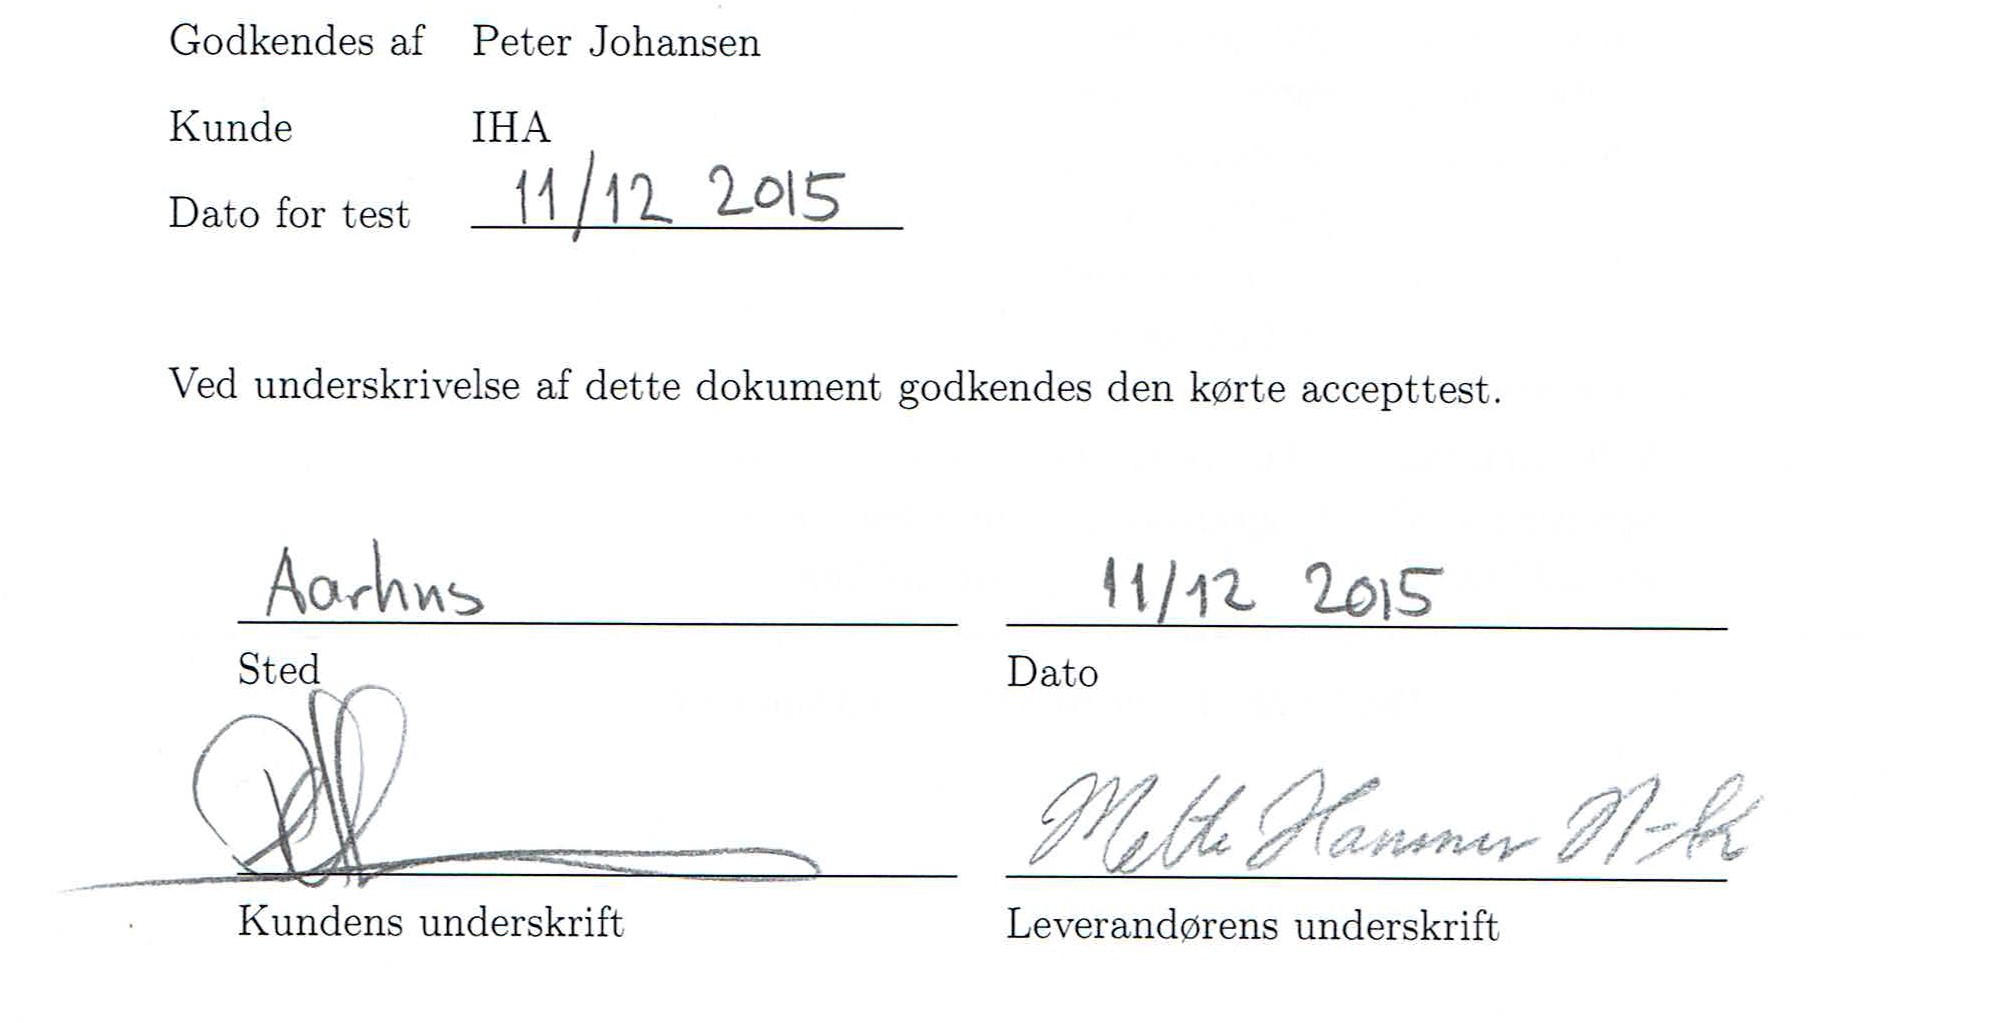
\includegraphics[width=1.0\textwidth]{Figurer/UnderskriftAT}
	%\caption{Udsnit af koden til det glidende middelværdifilter}
	%\label{fig:Kode udsnit af det glidende middelværdifilter}
\end{figure}



\newpage
\section{Problemrapport}
Use Case 3, handling 4: Systolisk og diastolisk blodtryk samt puls bliver vist i bokse på GUI. \\ 
Alle boksene er oprettet og vises i GUI, men kun systolisk og diastolisk bokse blive udfyldt. Puls er ikke kommet til at fungere. 

Ikke-funktionelle krav, handling 17: Grafen vises i ét vindue, hvor y-aksen måles i mmHg og x-aksen i tid i sekunder.\\
Y-aksen vises i mmHg, men x-aksen viser tid i antal samples. Dog passer det overens med at grafen viser 300 samples, så det vides at grafen viser 6 sekunder.  

Ikke-funktionelle krav, handling 21: Systemet skal kunne måle blodtryksværdier fra 0 til 250 mmHg. \\
Dette kan systemet også, det er blot blevet valgt ikke at sætte nogle begrænsninger på, så y-aksen med mmHg stopper ikke ved de 250 mmHg. Hvis dette ønskes kan det uden problemer tilføjes i koden, ved at låse grafområdets y-akse til at gå fra 0 til 250 mmHg.  